\documentclass{article}

\usepackage{amsmath}
\usepackage{amssymb}
\usepackage{tikz}

\begin{document}
\begin{enumerate}
\item[1.7.2]
  An equalizer $e : X \rightarrow A$ for arrows $f: A \rightarrow B$ and $g: A \rightarrow B$ has the properties:

  \begin{enumerate}
  \item $e;\ f = e;\ g$
  \item For every arrow $e^\prime: X^\prime \rightarrow A$ satisfying $1$, there exists a unique arrow $k: X^\prime \rightarrow X$ such that $k;\ e = e^\prime$.
  \end{enumerate}

  Universal constructions describe a class of objects and arrows sharing a common property and pick out the terminal objects when this class is considered as a category.
  For equalizers, the common property is that $e'; f = e'; g$ for a class of arrows, and the terminal objects are the equalizer arrows; that is, the $e$ with a unique arrow from every other $e'$.

\item[]
\item[1.7.4.1]
  First, we observe that a identity arrows are equalizers in a poset considered as a category because the dashed arrow $k = id_A$ is unique.
  \begin{center}
    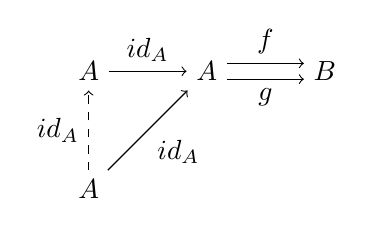
\begin{tikzpicture}
      \node (1) {$A$};
      \node[right of=1,xshift=0.5cm] (2) {$A$};
      \node[right of=2,xshift=0.5cm] (3) {$B$};
      \node[below of=1,yshift=-0.5cm] (4) {$A$};

      \draw[transform canvas={yshift=0.1cm},->] (2) -- node[above] {$f$} (3);
      \draw[transform canvas={yshift=-0.1cm},->] (2) -- node[below] {$g$} (3);
      \draw[->] (1) -- node[above] {$id_A$} (2);
      \draw[dashed,->] (4) -- node[left] {$id_A$} (1);
      \draw[->] (4) -- node[below right] {$id_A$} (2);
    \end{tikzpicture}
  \end{center}

  To prove that identity arrows are the only equalizers, assume have non-identity equalizer $e : A \rightarrow B$ for two functions $f,g : B \rightarrow C$.
  We know that $id_B$ is another equalizer of $f$ and $g$, so we must prove that there is a unique arrow $k : B \rightarrow A$ such that $e \circ k = id_B$.
  \begin{center}
    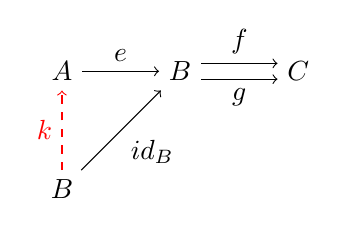
\begin{tikzpicture}
      \node (1) {$A$};
      \node[right of=1,xshift=0.5cm] (2) {$B$};
      \node[right of=2,xshift=0.5cm] (3) {$C$};
      \node[below of=1,yshift=-0.5cm] (4) {$B$};

      \draw[transform canvas={yshift=0.1cm},->] (2) -- node[above] {$f$} (3);
      \draw[transform canvas={yshift=-0.1cm},->] (2) -- node[below] {$g$} (3);
      \draw[->] (1) -- node[above] {$e$} (2);
      \draw[red,dashed,->] (4) -- node[left] {$k$} (1);
      \draw[->] (4) -- node[below right] {$id_B$} (2);
    \end{tikzpicture}
  \end{center}

  However, there is no such arrow.
  All arrows from an object $A$ to an object $B$ in a poset considered as a category have the property that $A \le B$ in the original poset.
  Hence if $e : A \rightarrow B$ exists then $k : B \rightarrow A$ cannot exist unless $A$ and $B$ are the same object.
  This is impossible unless $e$ is an identity arrow.
  Therefore the only equalizers in a poset considered as a category \emph{are} identity arrows.

\item[]
\item[1.7.4.2]
  Every equalizer $e : B \rightarrow C$ is monic because if we have arrows $k : A \rightarrow B$ and $k' : A \rightarrow B$ such that $e \circ k = e \circ k'$ then we are guaranteed that $k = k'$ because there is exactly one unique arrow from the object $A$ to the domain of the equalizer $e$.
  This follows because the arrows $k \circ e$ and $k' \circ e$ must also be equalizers (and any other equalizer must have a unique arrow to $e$).
  
\item[]
\item[1.7.4.3]
  
\end{enumerate}
\end{document}
